\Chapter{Nim játék és Northcott-sakk példaprogram}

\section{Felhasználói dokumentáció}
\subsection{Rendszerkövetelmények}
A program Java-ban íródott, éppen ezért futtatásához Java SE 1.8 futtatókörnyezet szükséges. A program nem támaszt különösebb rendszerkövetelményt a futtató géppel szemben, egy mai asztali számítógépen probléma nélkül el kell, hogy fusson. Legalább egy 1024x768-as felbontású monitor szükséges az ablak megjelenítéséhez, továbbá a programot egérrel, és billentyűzettel (vagy ezt kiváltó perifériákkal) lehet vezérelni.

\subsection{Telepítési útmutató}
A programot nem szükséges telepíteni, a Java archívumot (.jar) egyszerűen a Java futtatókörnyezetével elindítva a program futtatható.

\subsection{A program használata}
A programot elindítva az \myref{fig:fokepernyo} főképernyő fogad minket:\ujsor
\begin{figure}[ht]
	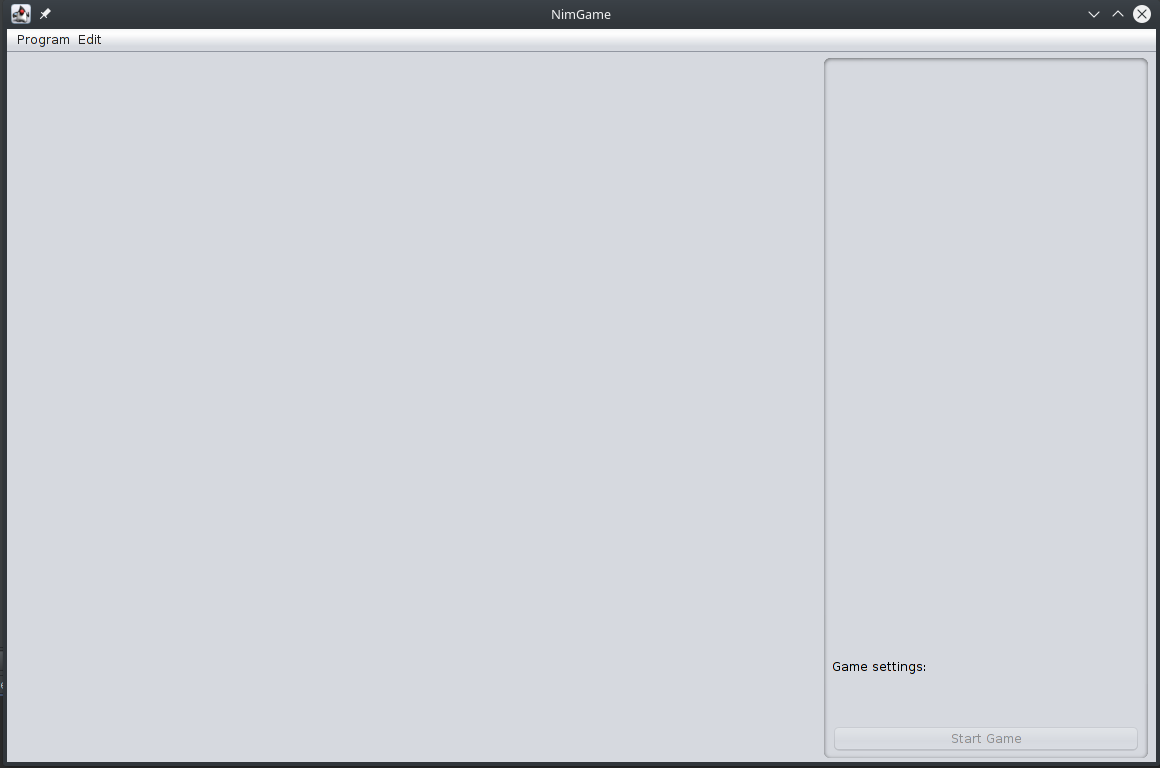
\includegraphics[width=10cm, height=8cm]{program/fokepernyo}
	\centering
	\caption{A példaprogram főképernyője}
	\label{fig:fokepernyo}
\end{figure}

A szoftver úgy lett megtervezve, hogy több különböző (nem feltétlenül csak Nim) játék futtatására legyen alkalmas, de alapvetően mindegyik játék három főbb elemmel rendelkezik. A beállításpanellel, az állapotpanellel, és a főpanellel. Az első kettő a jobb oldalon található oldalsó panelen jelenik meg, míg a főpanel az ablak nagyobb részét kitöltő üres helyen helyezkedik el, amint a megfelelő játékot betöltjük. \ujsor

Játékot betölteni a "Program" menü (\myref{fig:program_menu}) "Select game" almenü segítségével lehet megtenni. Itt ki kell választani a kívánt játékot. 
\begin{figure}[ht]
	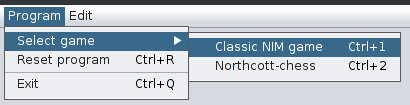
\includegraphics[width=8cm, height=2cm]{program/program_menu}
	\centering
	\caption{A főképernyő program menüje}
	\label{fig:program_menu}
\end{figure}


Jelenleg két játék közül lehet választani, ezeknek a leírására külön fejezetet szentelek. Az aktuális játékot bezárni a "Reset program" menüelemmel lehetséges, továbbá a programból kilépni az "Exit" menüelem használatával tud a felhasználó.\ujsor

Ezek a menüelemek a program futása során bármikor elérhetőek, azonban fontos megjegyezni, hogy amennyiben futó játék alatt egy másik játéktípus kerül kiválasztásra, abban az esetben az éppen játszott játék bezárásra kerül csak úgy, mintha a "Reset program" menüelemet választottuk volna.\ujsor

A legtöbb menüelemet gyorsbillentyű segítségével is aktiválni lehet. Hogy melyik elemhez milyen gyorsbillentyű tartozik arról a menüfelirat mellett elhelyezkedő billentyűparancs ad tájékoztatást.

\subsection{Klasszikus Nim Játék}
A klasszikus Nim - mint arra a neve is utal - a hagyományos Nim játék megvalósítása. Az \myref{fig:nim_ingame} ábra éppen azt mutatja, amint a gép ellen játszok. Jól látszik, hogy a játékban (éppen) 4 halom van, amelyekben a kavicsok darabszáma rendre 7, 9, 8, 7. Az állapotablakban jól látszik, hogy négy körön már túl is vagyunk.
\begin{figure}[h]
	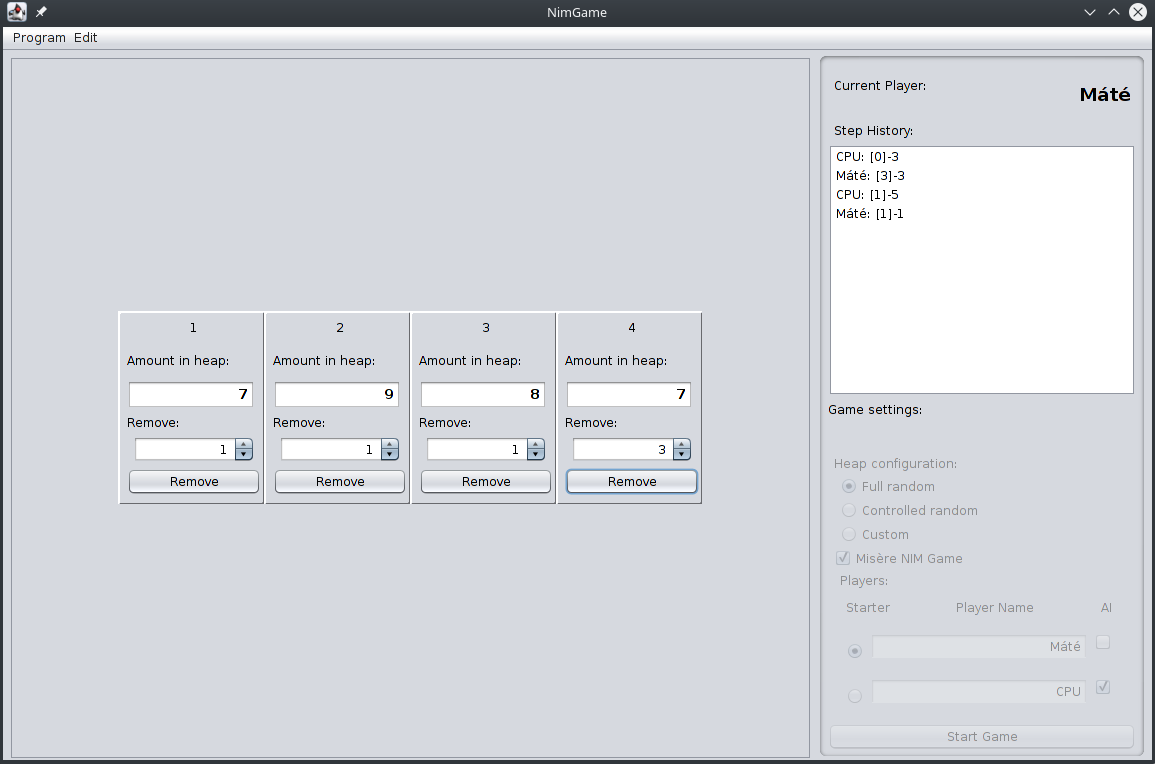
\includegraphics[width=14cm, height=10cm]{program/nim_ingame}
	\centering
	\caption{Klasszikus Nim játék a gép ellen}
	\label{fig:nim_ingame}
\end{figure}

A játék kezdete előtt lehetőségünk van részletekbe menően beállítani, hogy pontosan hogyan szeretnénk játszani a játékot. Ehhez be kell állítanunk a halom konfigurációt és a játékosokat. Miután a beállításokkal végeztünk az oldalsó panel alján található "Start Game" gombbal kezdhetjük a játékot. Ezután a beállítások módosítása már nem lehetséges, de bármikor kezdhető új játék a már említett menüelemek használatával.

\subsubsection{Játékos beállítások} \label{section:nim_playersettings}
A Nim játékot természetéből fakadóan két "személy" játssza. A szövegbeviteli mezőkbe a játékosok neveit kell megadni (eltérőeknek kell lenniük). A bal oldalon található rádiógomb segítségével azt választhatjuk ki, hogy melyik játékos kezdjen, még a jobb oldalon elhelyezkedő jelölőnégyzet arra szolgál, hogy tudassuk a programmal, hogy azt a játékost ő vezérli.\ujsor
A beállítások adta szabadságból látszik, hogy a programmal lehet ember-ember, gép-ember, és gép-gép játékot is játszani.

\subsubsection{Halom beállítások} \label{section:nim_gamesettings}
A halombeállítások kezdetén azt kell eldönteni, hogy milyen mélységben szeretnénk beleszólni a kezdeti játéktér felépítésébe. Ezt vezérelni a "Heap Configuration" szöveg alatti rádiógomb-csoporttal lehetséges. Ezekre kattintva a felület dinamikusan átalakul további funkciókat felfedve. 

\begin{itemize}
	\item Full random: Teljes egészében a programra bízzuk, hogy hány halmot generál milyen elemszámmal
	\item Controlled random: Továbbra is a gépre bízzuk, hogy összeállítsa a játékteret, azonban a generálás szabályokat ezzel vezérelni tudjuk. Erre kattintva a \myref{fig:nim_settings_controlledrandom} panel megjelenik, ahol az első sorban a halom számát, a második sorban a halmok elemszámára tudunk egyéni korlátot megadni. Az első oszlop az alsó korlátot, a második pedig a felső korlátot adja meg.
	\item Custom: Itt teljesen megszabjuk, hogy hány halmot szeretnénk milyen elemszámmal. Erre a gombra kattintva egy új panel (\myref{fig:nim_settings_custom}) jelenik meg, ami egy szövegbeviteli mezőből áll. A mezőbe szóközzel elválasztva kell megadni, hogy a halmokban hány elem legyen. Mindegyik szám egy halmot reprezentál, és a halmok az itt megadott sorrendben fognak létrejönni.
\end{itemize}

Amennyiben Misère Nim játék helyett normál módon akarunk játszani, akkor a "Misère NIM Game" jelölőnégyzetetek szüntessük meg a bejelöltségét.

\begin{figure}[h]
	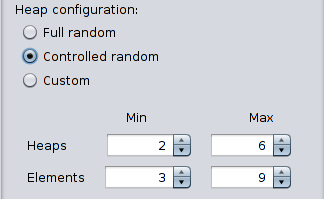
\includegraphics[width=5cm, height=3cm]{program/settings_controlled_random}
	\centering
	\caption{Irányított generálás}
	\label{fig:nim_settings_controlledrandom}
\end{figure}

\begin{figure}[h]
	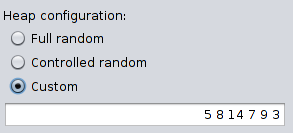
\includegraphics[width=5cm, height=2cm]{program/settings_custom}
	\centering
	\caption{Egyedi halomkonfiguráció}
	\label{fig:nim_settings_custom}
\end{figure}

\subsubsection{A játék menete}
Miután végeztünk a beállításokkal kattintsunk a "Start Game" gombra, és a játék elindul. Ekkor a jobb felső sarokban található állapotablak tájékoztat minket arról, hogy ki az éppen soron lévő játékos. \ujsor

A főpanelon látszódnak a halmok 1-1 panel formájában. Mindegyik panel tetején megtalálható a panel sorszáma, alatta egy szövegbeviteli mezőben a halomban található elemek száma, az alatt egy pörgettyűben beállítható az elvenni kívánt elemek darabszáma, majd legalul az elvesz gomb. \ujsor

Az éppen soron következő játékosnak meg kell hoznia megfelelő döntést, és lépnie kell oly módon, hogy a kiválasztott halomhoz tartozó pörgettyűbe beállítja mennyivel szeretné csökkenteni a halom elemszámát, és megnyomja a halomhoz tartozó "Remove" gombot. Ekkor a halom elemszáma csökken, a játékos köre véget ér, és a következő játékos kerül sorra. Amennyiben egy halom elfogy abban az esetben az azt reprezentáló panel eltűnik.\ujsor

A játék véget ér, amennyiben mindegyik halom elfogy, és a program egy előugró üzenetben ad tájékoztatást arról, hogy melyik játékos nyerte meg a játékot.

\subsection{Northcott-sakk}
\subsubsection*{A játék beállítása}
A Northcott-sakk sok tekintetben hasonlít a hagyományos Nim játékra, éppen ezért beállítása is hasonlóan történik. A szövegbeviteli mezőkbe a játékosnevet kell írni, a bal oldali rádiógomb kiválasztja a kezdőjátékost, míg a jobb kéz felől található jelölőnégyzet a játékost gépinek jelöli.\ujsor

Ami viszont lényeges eltérés, hogy itt a halom beállításai mások, mint a Nim esetében. A \myref{fig:northcott-settings} ábrát megfigyelve lényegesen leszűkültek a beállítási lehetőségek. Itt gyakorlatilag csak a sakktábla dimenzióját adhatjuk meg. A "Horizontal" (Vízszintes) az oszlopok számát, míg a "Vertical" (függőleges) a sorok számát adja meg. Ez nim játékra levetítve oszlop darab halom, és minden halomban maximálisan sor darab elem.

\begin{figure}[ht]
	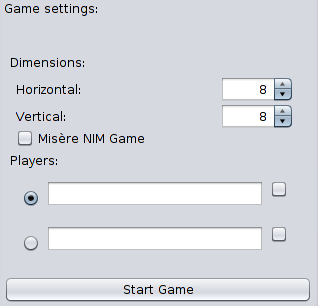
\includegraphics[width=5cm, height=5cm]{program/northcott-settings}
	\centering
	\caption{Northcott-sakk beállítópanelje}
	\label{fig:northcott-settings}
\end{figure}

Ez a játék is játszható Misère módon, a hozzá tartozó "Misère NIM Game" jelölőnégyzettel lehet állítani, hogy Misère, vagy normál módon kívánunk játszani.

Látható, hogy a véletlen halomgenerálás teljesen eltűnt. Ennek az az oka, hogy a játék kezdése előtt van egy extra művelet, ami nem teszi lehetségessé a véletlen generálást.

\subsubsection*{A játék előkészítése}
Ha végeztünk a játékbeállításokkal, akkor még ne indítsuk el a játékot, ugyanis a játékosoknak lehetőségük van beállítani a bábujuk kezdő pozícióját. A játéktér kezdetben mindkét játékos térfelét elfedi. A térfeleket az főpanel alján lévő két vezérlőgombbal lehet fel, illetve elfedni. A gép által vezérelt játékos bábuinak kezdőpozíciója nem állítható, így a hozzá tartozó gomb eltávolításra kerül, ha jelölőnégyzetet bejelöltük.\ujsor

\begin{figure}[ht]
	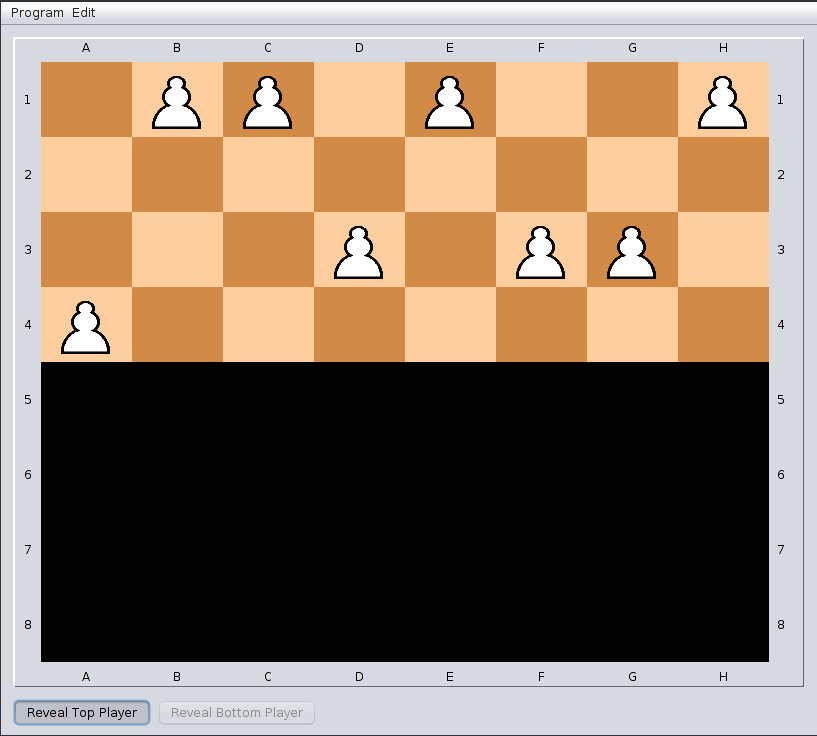
\includegraphics[width=8cm, height=8cm]{program/northcott-setup}
	\centering
	\caption{Northcott-sakk kezdő pozíciók beállítása}
	\label{fig:northcott-setup}
\end{figure}

A felső játékos - miután meggyőződött arról, hogy ellenfele nem figyeli - a "Reveal Top Player" gombra kattintva felfedi saját játékterét. Felfedett állapotba a gomb "beragad", és a másik gomb letiltódik, hogy véletlenül ne lehessen az ellenfél térfelére átváltani. A felső játékos a kívánt mezőre kattintva áthelyezheti az adott oszlopban lévő bábuját arra a mezőre, amelyikre kattintott. Ha a felső játékos késznek érzi a kezdőállapotot, akkor a beragadt gombra újból rákattintva elfedi a felső játékteret, és átadja a helyét az alsó játékosnak, aki ugyanezt a műveletsort végigjátssza. \ujsor

Miután mindketten végeztek a beállítással, a játék a "Start Game" gombra kattintva indítható. Ezután a játék beállításai már nem módosíthatóak, a beállításhoz tartozó vezérlőelemek letiltásra, a játéktér elrejtéséért/felfedéséért felelős vezérlőgombok eltávolításra kerülnek.


\subsubsection*{A játék menete}
A játék indulásakor a teljes játéktér felfedésre kerül, és a program a jobb felső sarokban található állapotpanelen tájékoztat a soron következő játékos kilétéről. Lépni úgy lehet, hogy a kiválasztott oszlopban arra a mezőre kattintunk, ahova a saját bábunkkal lépni szeretnénk. A mezőre kattintva a lépés bekövetkezik, és a játékos köre véget ér, helyére a következő játékos lép.\ujsor

\begin{figure}[!ht]
	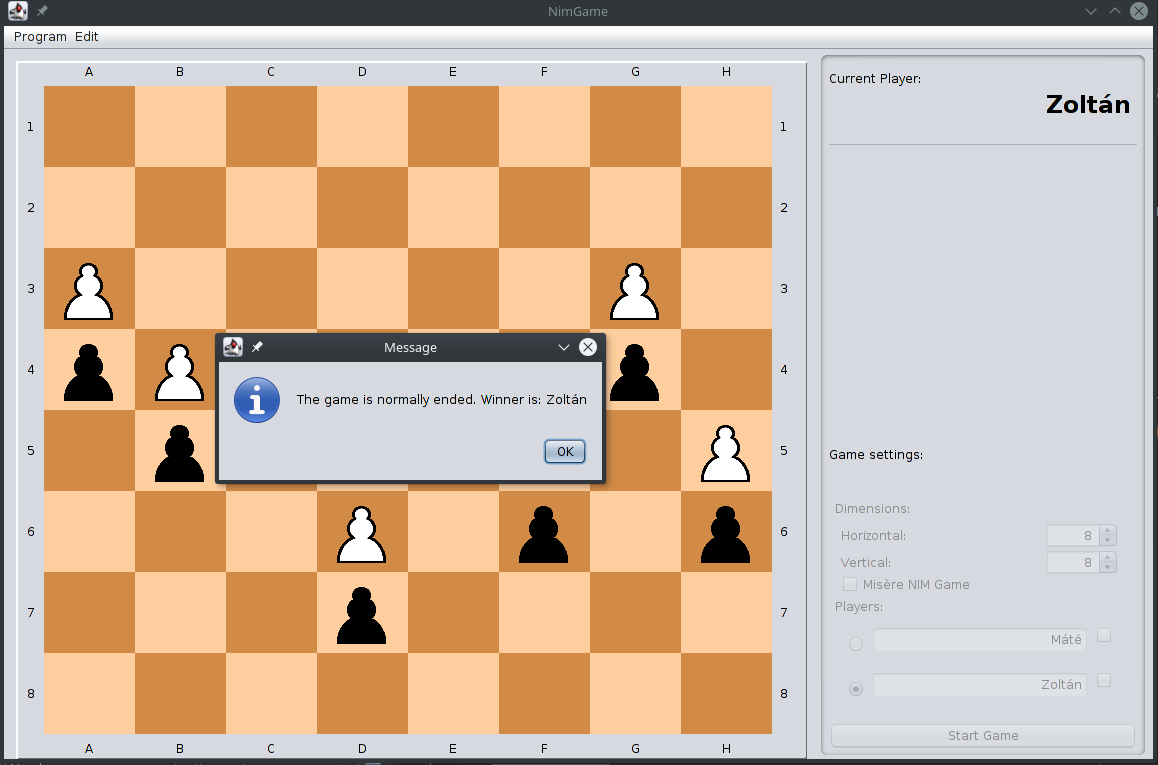
\includegraphics[width=12cm, height=8cm]{program/northcott-end}
	\centering
	\caption{Northcott-sakk játék vége; nyertes játékos Zoltán}
	\label{fig:northcott-end}
\end{figure}

A játék addig tart, amíg van olyan oszlop, ahol a bábuk között lévő távolság nagyobb, mint 0, azaz nem közvetlenül egymás mellett áll mindegyik bábu. A játék végén a program egy előugró ablakban ad tájékoztatást arról, hogy a játékot melyik játékos nyerte meg.


\section{Fejlesztői dokumentáció}

Általánosságban elmondható, hogy amikor az ember találkozik egy konkrét problémával, az gyakran egy nagyobb, összetettebb problémakör része. Éppen emiatt amikor egy megoldandó problémával kerülök szembe, első körben sosem az adott problémára koncentrálok, hanem próbálom megtalálni mi az a kiinduló pont, ahonnan a probléma valójában eredeztethető. Ennek meg van az a hátránya, hogy sokszor lényegesen több munkát kell belefektetni abba, hogy a konkrét problémát megoldjuk, ugyanakkor a megoldás sokkal több problémára nyújt megoldást, s később nagyságrendekkel könnyebben lehet adaptálódni a változó igényekhez. A saját tapasztalataim is azt mutatják, hogy egy adott problémára adandó megoldás követelményei kezdetben egészen mások, mint amire végül szükség van.\ujsor

Nem volt ez most sem másképp. Eredeti megközelítésemben egy univerzális játékmotort képzeltem el, ahol a játékok maguk csupán kiegészítései a szoftvernek, amiket a felhasználók - akár futásidőben is - készíthetnek, vagy módosíthatnak. Ehhez a játékmotorhoz tartozott volna egy univerzális gépi játékos is, ami a játékleíróban található szabályok szerint játszott volna. Ez az elképzelés nagyon szép, ugyanakkor rengeteg időt vett volna igénybe, ami nem állt a rendelkezésemre, így ezt tervet végül végletekig leegyszerűsítettem. Egy dologból azonban nem engedtem. A játékok most is különálló modulként viselkednek (csak bele vannak "égetve" magába a játékmotorba), és erre nagyon jó okom volt.\ujsor

Nem célom a teljes forráskód beillesztése a dolgozatba, mert egyrészt viszonylag nagy méretű, (több ezer sor) sok rész triviális, vagy csak technikai, azonban bizonyos osztályokat, vagy kódrészleteket behivatkozok, amikben úgy érzem, hogy említésre méltó dolgok találhatóak.

\section{Program felépítése, tervezési szempontok} \label{section:implementation_design}
Kezdetektől fogva a Northcott-sakkot szerettem volna leimplementálni, ugyanis a Nim játékok variánsai közül látványosabbak közé tartozik, és nagyon tetszett az a tulajdonsága, hogy egy-az-egyben visszavezethető hagyományos Nim játékra. Ebből következően az implementálást nem is a Northcott-sakkal kezdtem, hanem a hagyományos Nim játékkal. Miután ezzel végeztem, akkor tértem át magára a szakdolgozatom gyakorlati feladatára, a Nortcott-sakkra. A visszavezethetőség szemléltetésére implementálás során különös figyelmet szenteltem, olyan szinten, hogy a Nortcott-sakk nem is különálló játékmodulként szerepel (ezzel kissé megszegve a program koncepcióját), hanem csupán egy új megjelenítési réteget ad a Nim játékhoz. Más szóval, amikor a felhasználó Northcott-sakkot játszik, akkor valójában a gép azt Nim játékként fogja fel. Konkrétan ugyanazt az osztályt (NimGameCore) használja felel a Nim játék, mint a Nortcott-sakk. Szándékosan még csak le sem származtattam, ezzel is kidomborítva a a Nortcott-sakk eme érdekes tulajdonságát.\ujsor

A programot Java nyelven írtam, és használok benne olyan nyelvi elemeket, amik megkövetelik a 8-as verziót, azonban a SE (Standard Edition) eszközkészletén túlmenően semmilyen egyéb külső programkönyvtárat nem használtam fel.\ujsor

A program belépési pontja a MainWindow osztályban található, ami gyakorlatilag létrehozza az alkalmazás főképernyőjét. A főképernyő áll egy menüsorból, egy oldalsó panelből, és egy főpanelből. A főpanelen helyezkedik el a létrehozott játék játéktere, míg az oldalsó panelen a létrehozott játék állapotpanelje, és a beállításpanelje. Ezek a panelok nem feltétlenül kell, hogy a java.swing.JPanel osztályból származzanak. Minden olyan komponenst be tud illeszteni ezekre a helyekre, amelyek a java.awt.Component osztályból származnak.\ujsor

Minden játék két részből tevődik össze. Egyrészt magából a játékból, amely a GameCore osztályból kell, hogy származzon, másrészt egy olyan osztályból, amely megvalósítja a GameEntityProvider interfészt. Ez az interfész nyújt lehetőséget arra, hogy az adott játék beállításait lekérdezzük, továbbá ez az interfész kiterjeszti a GameUIProvider osztályt ami segítségével a már említett játék-specifikus komponenseket lehet lekérdezni. A játékot, és a GameEntityProvider-t a GameController osztály fogja össze, és egységesen egy játékként kezeli. Amennyiben egy futó játékot szeretnénk terminálni ezt rajta keresztül kell megtenni, ez gondoskodik a játék leállításáról, és a grafikus vezérlőelemek helyreállításáról.\ujsor

A játékok felépítése hierarchikus. Mindegyik játék abból az osztályból származtat le, amelyik leginkább megfelel neki. Az alaposztály a GameCore, ami általános koncepciókat tartalmaz egy játékról mindenféle specializáció nélkül. A következő szint a TurnBasedGame, ami a körökre osztott játékok használhatnak, és jelenleg erre épül a NimGameCore. Mindegyik hierarchia hozhatja magával az adott szinthez tartozó kiegészítő (esemény, kivétel) osztályokat.

\section{Objektumok közti kommunikáció}
Fontos rögtön az elején tisztázni, hogy a program jelenleg egy szálra van felkészítve, azaz sem a metódusok, sem pedig az algoritmusok nem szál-biztosak, nincsenek felkészítve a többszálú futásra, a hívások szinkron módon történnek. Ez jelenleg - a program egyszerűségéből fakadóan - nem okoz nagy problémát, egyetlen kellemetlenség van csupán, abban az esetben, ha két gépi játékost játszatunk egymás ellen, kellően nagy játékteret biztosítva számukra, akkor amíg a játékot játsszák a felhasználói felület az eseményekre nem reagál.\ujsor

Kommunikációra kétféle módszert használunk. Általában ha egy esemény több objektumból érkezhet, de a célja mindig egy konkrét objektum, akkor ott interfészt definiálunk. Egyes esetben - ha a kommunikáció két irányú - nem is egyet, hanem mindjárt kettőt a vissza-irányba is. Amennyiben egy eseményt potenciálisan több helyre szeretnék eljuttatni, akkor az EventManager szolgáltatásait vesszük igénybe.

\subsection{A program eseménykezelője}
A programban egy nagyon pici, egyszerű eseménykezelőt implementáltam, a továbbiakban részletezem a felépítését, és használatát.

\subsubsection{EventManager}
Az EventManager egy nagyon pici statikus osztály, aminek az a feladata, hogy - igény esetén - EventChanneleket létrehozzon, a létrehozott EventChanneleket nyilvántartja, és igény esetén ezeket az objektumokat kérésre átadja, illetve ha egy EventChannel tulajdonosa úgy dönt, hogy megszünteti az EventChannelt, akkor ezen keresztül teheti meg ő, és csakis ő.

\subsubsection{EventChannel}
Az EventChannel feladata, hogy egyfajta csatornaként működjön. Erre a csatornára bárki feliratkozhat a subscribeForChannel(GameEventListener eventListener) metódus használatával. Paraméterben a feliratkozónak meg kell adnia önmagát, továbbá implementálnia kell a GameEventListener interfészt, ami gyakorlatilag egy visszahívó metódust tartalmaz. A visszahíváskor két paraméter adódik át. A csatorna azonosítója, illetve az eseményobjektum, ami a GameEventből kell, hogy származzon.

\subsubsection{GameEvent}
A GameEvent a játék eseményeinek az alaposztálya. Gyakorlatilag egy fontos dolgot tárol, hogy az esemény honnan származik. Minden kiegészítő információ tárolása a leszármaztatott objektumra van bízva. A GameEvent jelen dokumentáció írásakor még tartalmaz egy típus mezőt is, azonban azt fontolgatom, hogy ezt koncepciót kiveszem az eseményből, és az esemény típusát maga az objektum osztálya határozza meg.\ujsor

Mint azt már korábban említettem a játékok követnek egyfajta hierarchiát, ami az eseményobjektumokon is megmutatkozik. Például a Nim játékok eseményeinek az alaposztálya a NimGameEvent, ami a TurnbasedGameEvent osztályból származik (ez adja hozzá a következő kör eseményt), ami pedig végül a GameEvent osztályból származik le.

\section{Az absztrakt játék (GameEngine) szintje}
Ez a program rétegződésének a legfelső szintje, gyakorlatilag minden osztálya absztrakt. Az itt található osztályok teljesen általánosan fogják fel a játék mibenlétét, ebből következően ezekből példányosítani értelmetlen, emiatt absztraktként vannak megjelölve. Mindazonáltal már ezen a szinten is bizonyos dolgokat ismerünk. Tudjuk például, hogy a játékot játékos(ok) játsszák, azok lépéseket tesznek meg, a játéknak van eleje, vége, és beállításai.

\subsection{StepObject}
Minden játékban léteznek valamiféle átmenetek, amik a játékteret a kezdőállapotból további állapotba, végül pedig a végállapotba viszik. Ezeket az állapotátmeneteket a StepObject objektumok reprezentálják. Az alap StepObject absztrakt osztály önmagában csak azt az információt tartalmazza, hogy ezt az átmenetet melyik játékos vitte véghez. Értelemszerűen a konkrét játéknak ki kell egészíteni ezt az osztályt a játék állapotátmeneteire vonatkozó információkkal.

\subsection{Player}
Egy tetszőleges játékost ír le ez az osztály. Ezen a szinten amit biztosan tudunk, hogy a játékosnak van egy neve, egy belső azonosítója, és egy PlayerControllerje, akitől szükség esetén lekérdezhetjük a játék beállításait, illetve a kontrolleren keresztül a játékot utasíthatjuk a következő lépés megtételére.

\subsection{GameCore}
Egy általános célú játék absztrakt megvalósítása. Nyilvántartja a játékosokat, eltárolja a lépéselőzményeket, a játék beállításait fogadni tudja, továbbá fenntart egy EventChannelt amire a program többi komponense feliratkozhat. A játék eseményeit ezen keresztül szórja szét.

\subsection{AbstractGameSettings}
Egy teljesen üres osztály, a játék beállításait tartalmazza, minden játéknak implementálnia kell a saját beállításait, melynek ebből az osztályból kell származnia.

\section{Nim játék leírása}
A Nim játékot megvalósító osztály a már említett NimGameCore. Az osztály, és a hozzá tartozó egyéb osztályok a gameplayer.nimgame.standard csomagban találhatóak.

\subsection{NimPlayer}

\subsubsection{NimHumanPlayer}
A NimHumanPlayer az emberi játékos implementációja. Gyakorlatilag egy üres implementáció, a cselekvés a felhasználói felületre van rákötve.

\subsubsection{NimAIPlayer}
Sokkal érdekesebb a NimAIPlayer osztály. Ez a gépi játékot megvalósító játékos implementációja. Látszik, hogy már egyből a konstruktorba létrehozom a mesterséges intelligenciát az adott játékospéldányhoz. Ez persze azt is jelenti, hogy több gépi játékos esetén több mesterséges intelligencia jön léte, ami magában hordozza annak a lehetőségét, hogy különböző MI implementációkat versenyeztessünk egymással.\ujsor

A notifyYourTurn() visszahívó metódusban értelemszerűen meghívom a mesterséges intelligencia getNextStep() metódusát, ami egy NimAISolution objektumot tartalmaz. Ezután már nincs más dolgom mint ezt az objektumot felhasználva készítsek egy NimStepObject objektumot, és a kontrolleren keresztül léptessem a gépi játékost. A mesterséges intelligenciát megvalósító osztályok a gameplayer.nimgame.standard.AI csomagban találhatóak, de erről részletesebben a \ref*{section:nim_impl_winning_strategy} részben írok.

\subsection{NimGameSettings}
A Nim játék lehetséges beállításait tartalmazza. A \ref*{section:nim_gamesettings} és a \ref*{section:nim_playersettings} pontokban részletesen leírtam a programomban lévő Nim játék nyújtotta lehetőségeket. Ezeknek a lehetőségeknek a megvalósítása szerepel ebben az osztályban.

\subsection{NimStepObject}
A Nim játék leszármaztat az alap StepObject osztályból hozzáadva azt az információt, hogy az adott lépésből melyik halomból mennyi elemet vett el az állapotátmenetet előidéző játékos.

\subsection{A Nim játék grafikus felhasználói felületelemei}
A Nim játék grafikus elemeit a gameplayer.nimgame.standard.UI csomagban találjuk. A \ref*{section:implementation_design} szekcióban már leírtam, hogy legalább három grafikus komponenst kell a játékoknak implementálni, és itt ez a három komponens a NimMainPanel, NimSettingsPanel, és a NimStatusPanel.

\subsubsection{NimMainPanel}
Egy javax.swing.JPanel típusú grafikus komponens. Ez valósítja meg a játékteret, de egy összefogó szerepe is van. Implementálja a GameEntityProvider interfészt, és a segédpaneleket is lepéldányosítja, továbbá feliratkozik a Nim játék EventRegistry osztályban található EVENT\_GAMEENGINE eseménycsatornára. Ennek köszönhetően a játéktérben bekövetkezett változásról azonnal értesül, és frissíteni tudja a játékteret.

\section{Northcott játék leírása}
A Northcott-sakk megvalósításának a szépsége, hogy ehhez a játékhoz nem tartozik játék, azaz nincsen hozzá olyan osztály, ami a GameCoreból származik le. Az egész játék csupán felhasználói felületelemekből épül fel - mint korábban írtam - a Nim játéknak ténylegesen csak egy másfajta megjelenítése.\ujsor

A három panel itt is ugyan úgy megtalálható: NorthcottMainPanel, NorthCottSettingsPanel, és NorthcottStatusPanel. Itt is a főpanel látja el az összefogó szerepét. Sok szempontból analóg a viselkedése a Nim játék főpaneljével, így részletesen ezt nem is tárgyalom.\ujsor

Akad azonban egy érdekes probléma. Az igaz ugyan, hogy a Northcott-sakkot vissza lehet vezetni a Nim játékra, ez fordítva azonban nem teljesen igaz. A Nim játékban a halmok elemszáma megfeleltethető ugyan a Northcott-sakkban a bábuk közt lévő távolságnak, azonban a bábuk pozíciójára vonatkozóan a Nim játék nem hordoz információt. Ezt a problémát áthidalandó az oszlopok nyilvántartanak egy eltolás értéket, ami azt mutatja meg, hogy a felső játékos bábuja a tábla tetejéhez képest mennyivel van lejjebb. Ehhez az eltolási értékhez hozzáadva a halom elemszámát megkapjuk az alsó játékos bábujának a helyét.

\section{Nim nyerő stratégia gépi implementációja} \label{section:nim_impl_winning_strategy}
A gépi játékost stratégiáját a AINimWinningStrategy osztály valósítja meg, amely implementálja a NimAI interfészt:
\lstinputlisting[language=java]{source/nimgame/standard/AI/NimAIStrategy.java}

A visszaadott NimAISolution objektum gyakorlatilag egy tárolóobjektum amely a kiválasztott halmot, és az abból elvett elemszámot tartalmazza.

Maga a stratégia implementációja jól követi az elméleti részben tárgyalt stratégiát, de néhány helyen magyarázatot igényel. \ujsor
A belépési pont a getNextStep() metódus, ami paraméterben megkapja a halomlistát. Ezután ezt átalakítja tömbbé, és meghívja a getBestMove() metódust. Az átalakítás nem szükséges, de az adatstruktúrán igen sok műveletet hajt végre az algoritmus, így optimálisabb ezzel az átalakítással.\ujsor
A getBestMove() a gerince a stratégiának, itt dől el, hogy a mesterséges intelligencia melyik lépést választja a következőnek. Először is megkeresi az első nem üres halmazt, (ha mindegyik halmaz üres, akkor dobunk egy kivételt, az MI nem futtatható üres játéktéren) majd egyszerű próbálkozással nekiáll megkeresni az első olyan állapotot, amit a DecisionMaker elfogad. Minden halomra (ha nem üres) megpróbálja elfogadtatni az lépést úgy, hogy először elvesz az aktuális halomból egyet, majd kettőt, és így tovább amíg el nem fogy a halom. Ha az egész halmot elvette, de még mindig nem fogadta el a lépést a DecisionMaker, akkor visszaállítja a halom elemszámát a kísérletezés előtti állapotra, és lép a következő halomra.\ujsor
A DecisionMaker egy belső interfész, melyet két belső osztály implementál. Feladata az, hogy eldöntse, hogy az éppen vizsgált lépés elfogadható-e legjobb lépésnek. Az a két belső osztály ami implementálja az pont a NimStandardDecisionMaker, és a NimMisereDecisionMaker. Mint a nevükből kiderül az egyik a hagyományos Nim játéknál hoz döntést, míg a másik a Misère módhoz. Első megközelítésben nem sok értelme látszik ennek a fajta megoldásnak, hiszen ezt a vizsgálatot beleépíthettem volna a kereső algoritmusba, azonban ha így tettem volna, akkor minden ciklusfutáskor kellett volna tennem egy feltételvizsgálatot, hogy éppen melyik módban van a játék. Így azonban a konstruktorban elvégzem ezt a vizsgálatot, és a mezőhöz a megfelelő DecisionMaker objektumot rendelem hozzá, így a ciklusban az összes ilyen vizsgálat elhagyható tovább gyorsítva az algoritmust.\ujsor
Ez az algoritmus majdnem minden esetben talál nyerő állapotot, kivéve, ha az ellenfél kezdett, és hibátlanul játszik. Ebben az esetben nem tud mit csinálni, így - mivel nincs jó megoldás, de lépni kell - elvesz az első nem üres halomból halomból egyet.

\lstinputlisting[language=java]{source/nimgame/standard/AI/AINimWinningStrategy.java}

